\section{Introduction}
\label{sec:intro}

Reported COVID-19 cases are a staple in tracking the pandemic at varying
geographic resolutions \citep{dong2020interactive, nyt2020corona,
wp2020tracking}. Yet, for every case that is eventually reported to public
health, several infections are likely to have occurred, and likely much earlier.
To see why, it is important to understand \emph{whose} cases are being reported
and what differentiates them from unreported cases as well as \emph{when} these
case reports happen. \Cref{fig:chain_events_onset_report} shows an idealized
path of a symptomatic infection that is eventually reported to public
health. This figure illustrates a number of sources of bias in the
reporting pipeline. For instance, diagnostic testing mainly targets symptomatic
individuals; thus, infected individuals exhibiting little to no symptoms are
omitted \citep{cdc2022estimated}. In addition, testing practices, availability,
and uptake vary temporally and spatially \citep{pitzer2021impact,
ecdc2020strategies, hitchings2021usefulness}. Finally, cases provide a belated
view of the pandemic's progression, because they are subject to delays due to
the viral incubation period, the speed and severity of symptom onset, laboratory
confirmation, test turnaround times, and eventual submission to public health
\citep{pellis2021challenges, wash2020dash}. For these reasons, reported cases
are lagging indicators of the course of the pandemic. Furthermore, they do not
represent the actual number of new infections that occur on any given day based on
exposure to the pathogen. Since there was no large-scale surveillance effort in
the United States that reliably tracked symptom onset, let alone infection
onset, ascertaining the onset of all \emph{infections} is challenging.

\begin{figure}[H]
\centering
    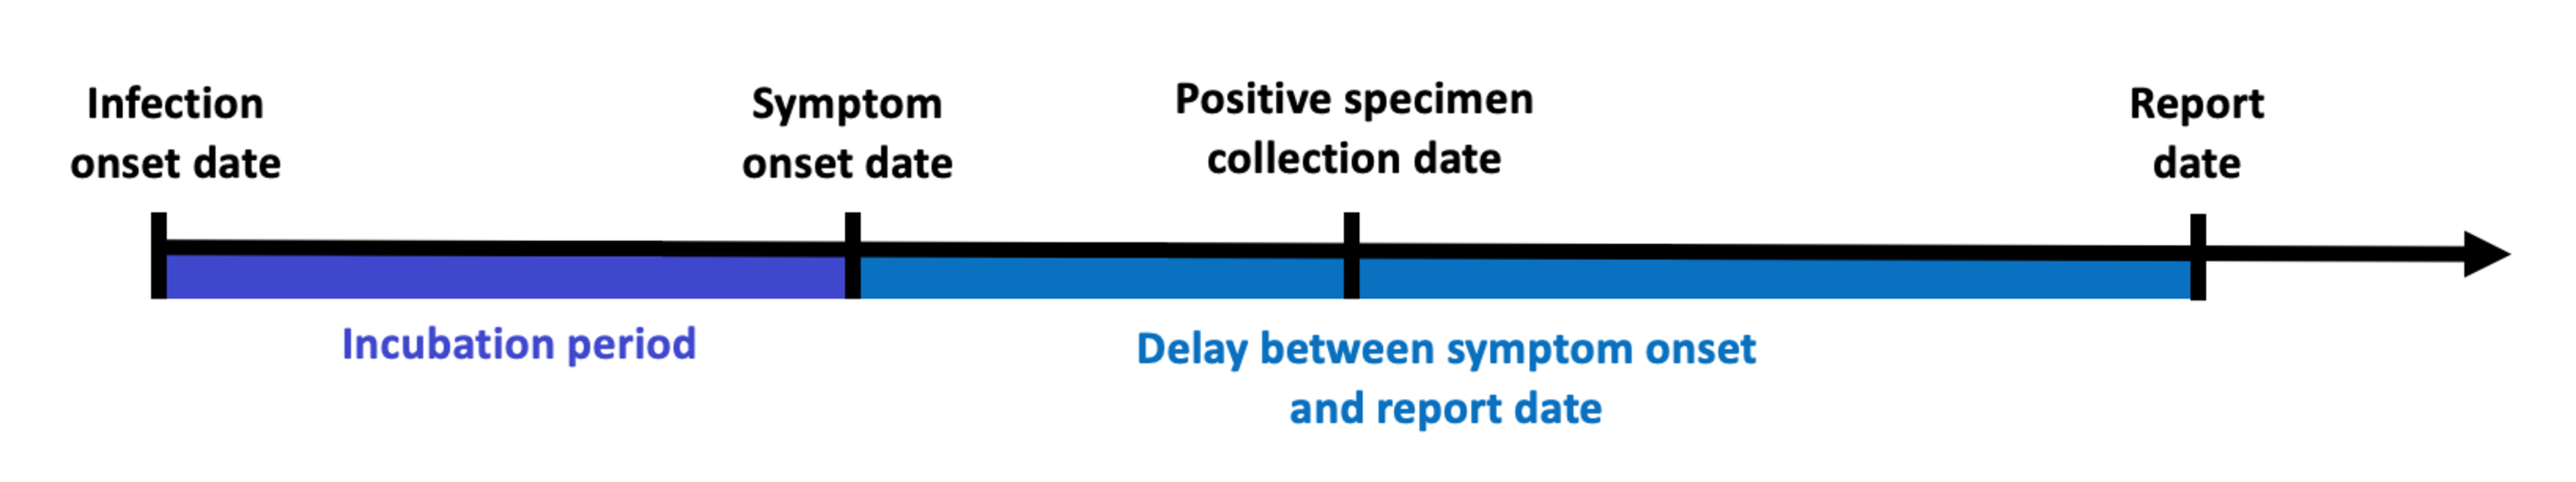
\includegraphics[width=.99\textwidth]{Chain_of_events_onset_report.pdf} 
    \caption{Idealized chain of events from infection onset to case report date 
    for a symptomatic infection that is eventually reported to public health.}
    \label{fig:chain_events_onset_report}
\end{figure}

% Importantly, all of these issues that are present in local health authority
% data are also present in the gold standard for case data from the JHU CSSE
% \citep{dong2020interactive, guidotti2022worldwide} because JHU scrapes case
% data from the local health authority dashboards \citep{jahja2022real}.
% Furthermore, the cases shown on the JHU CSSE Coronavirus Resource Center
% \citep{jhucsse2020covid} are those that have been disseminated to the public
% on a given day. 
% Our approach to estimate latent infections takes case data and estimates the 
% following...

Contextualizing the course of the pandemic, understanding the effects of
interventions, and drawing insights for future pandemics is challenging because
the spatial and temporal behaviour of infections is unknown. While reported
cases provide a convenient proxy of the disease burden in a population, it is
incomplete, delayed, and misrepresents the true size and timing of the pandemic.
Regardless of these difficulties, it is important to the public and to public
health to perform a pandemic post-mortem. Estimates of daily incident infections
are one such way to measure this and can guide understanding of the pandemic
burden over space and time. 

\begin{figure}[H]
\centering
    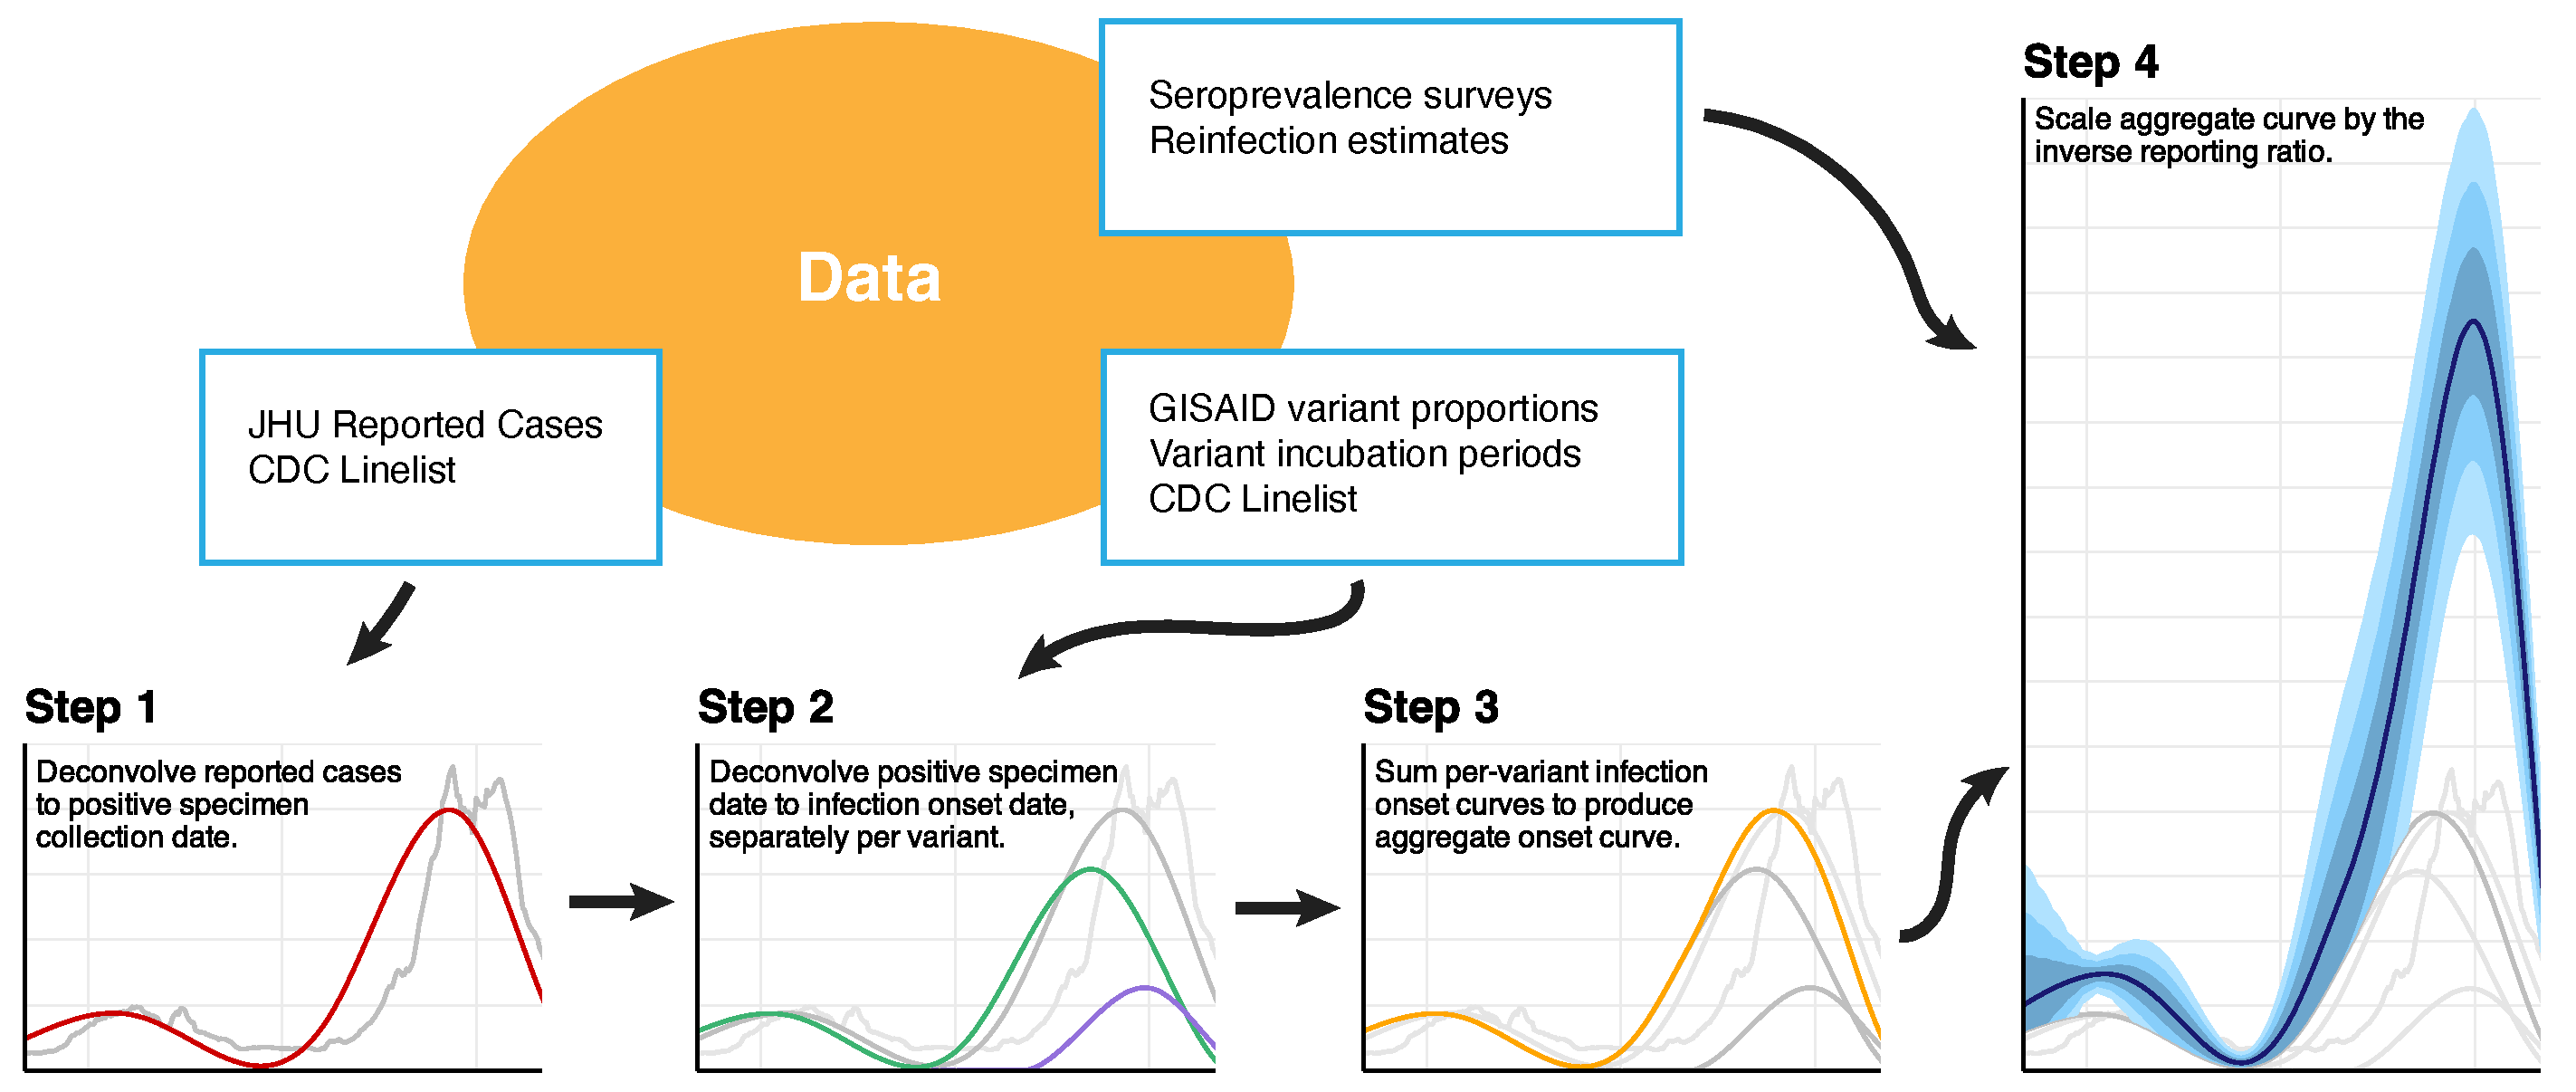
\includegraphics[width=.9\textwidth]{li-flowchart.pdf} 
    \caption{Flowchart of the data and major analysis steps required to get from
    reported cases to incident infection estimates. In Step 1, we use the CDC
    line list data to deconvolve reported cases (grey) backward to the date of
    positive specimen (red). Step 2 separately deconvolves these to the date of
    infection by variant (Epsilon in Purple, Ancestral in Green), 
    before summing across all variants (orange)
    in Step 3. Finally, we use seroprevalence
    survey and time-varying reinfection data to account for the unreported
    infections.}
    \label{fig:cases_to_infect_flowchart}
\end{figure}
    

In this work, we provide a data-driven reconstruction of daily incident
infections for each \US state before the onset of Omicron. Using
state-level line list data, we estimate state-date specific distributions for
the delay from symptom onset to positive specimen date and positive specimen to
case report date. We combine these with variant-specific incubation period
distributions to deconvolve daily reported COVID-19 cases back to their
infection onset, removing the effects of the delays. Finally, we adjust for
unreported infections with seroprevalence and reinfection data, accounting for
the waning of antigenic immunity over time. A graphical depiction of our
procedure is shown in \Cref{fig:cases_to_infect_flowchart}. Our results examine
features of our infection estimates and the implications of using them, rather
than reported cases, to assess the impact of the pandemic. We also produce
simple time-varying infection-hospitalization ratios (IHRs) for each state and
compare these with case-hospitalization ratios (CHRs). While these analyses
provide a glimpse into the utility of our infection estimates, we believe that
there is much more to be explored, and we hope that our work serves as a
benchmark for future retrospective analyses. 

